\documentclass[a4paper,12pt]{article}
\usepackage[utf8]{inputenc}
\usepackage{geometry}
\geometry{margin=1in}
\usepackage{amsmath}
\usepackage{booktabs}
\usepackage{array}
\usepackage{enumitem}
\usepackage{graphicx} % For \resizebox
\usepackage{graphicx} % For \includegraphics
\usepackage{float} % For [H] placement
\begin{document}

\title{Efficient CPU Design with Multiple Addressing Modes}
\author{} % Add your name here if needed
\date{} % Explicitly set to empty to suppress date
\maketitle

\section{CPU Structure Selection}
\textbf{Choice:} Register-based CPU Architecture \\
\textbf{Justification:} A register-based CPU offers flexibility and efficiency compared to accumulator-based (limited to one register) and stack-based (reliant on memory-intensive push/pop operations) designs. Registers reduce memory access latency by storing intermediate results, improving execution speed. Modern CPUs (e.g., x86, ARM) predominantly use register-based designs due to their balance of performance and scalability. \\
\textbf{Instruction Flow in Pipeline:} The CPU uses a 5-stage pipeline (Fetch, Decode, Execute, Memory Access, Write-back). Registers facilitate operand access in the Execute stage, minimizing memory stalls.

\section{Instruction Format Design}
\textbf{Proposed Format:} A 32-bit instruction word supporting zero, one, two, and three-addressing modes. \\
\textbf{Structure:}
\begin{itemize}
    \item \textbf{Opcode (6 bits):} Identifies the operation (e.g., ADD, LOAD, JMP), supporting up to 64 instructions.
    \item \textbf{Addressing Mode Flags (2 bits):} Specifies the mode (00: Immediate, 01: Direct, 10: Indirect, 11: Indexed).
    \item \textbf{Register Fields (3 $\times$ 5 bits):} Three 5-bit fields (R1, R2, R3) for source/destination registers (up to 32 registers).
    \item \textbf{Immediate/Offset Field (9 bits):} Used for immediate values or memory offsets in applicable modes.
\end{itemize}
\textbf{Supported Addressing Modes:}
\begin{itemize}
    \item \textbf{Zero-address:} Stack-like operations (e.g., \texttt{ADD} pops two operands, pushes result).
    \item \textbf{One-address:} Accumulator-like (e.g., \texttt{LOAD R1} loads into R1).
    \item \textbf{Two-address:} Register-to-register (e.g., \texttt{ADD R1, R2} $\rightarrow$ R1 = R1 + R2).
    \item \textbf{Three-address:} Full flexibility (e.g., \texttt{ADD R1, R2, R3} $\rightarrow$ R1 = R2 + R3).
\end{itemize}
\textbf{Optimization:} Variable-length encoding is avoided to simplify fetch/decode stages, reducing pipeline delays. The 32-bit fixed format balances flexibility with fetch efficiency.

\section{Integration of Addressing Modes}
\begin{itemize}
    \item \textbf{Immediate:} Data is embedded in the instruction (e.g., \texttt{MOV R1, \#5}). Fast but limited by the 9-bit field size.
    \item \textbf{Direct:} Memory address is specified (e.g., \texttt{LOAD R1, 0x100}). Simple but requires memory access.
    \item \textbf{Indirect:} Address is in a register (e.g., \texttt{LOAD R1, [R2]}). Flexible for pointers but adds a register fetch cycle.
    \item \textbf{Indexed:} Base register + offset (e.g., \texttt{LOAD R1, [R2 + 4]}). Ideal for arrays, balancing speed and complexity.
\end{itemize}
\textbf{Trade-offs:}
\begin{itemize}
    \item \textbf{Speed:} Immediate is fastest; Indirect/Indexed add latency due to additional fetches.
    \item \textbf{Memory Efficiency:} Direct/Indexed use memory efficiently for large data; Immediate wastes bits for small values.
    \item \textbf{Complexity:} Indirect/Indexed increase control unit complexity but enhance flexibility.
\end{itemize}

\section{Control Unit Design}
\textbf{Type:} Hardwired control unit for speed, with microprogrammed fallback for complex instructions. \\
\textbf{Functions:}
\begin{itemize}
    \item \textbf{Instruction Decoding:} Parses opcode and addressing mode flags, routing signals to ALU, registers, or memory.
    \item \textbf{Execution Flow:} Manages pipeline stages, resolving hazards (e.g., data dependencies) with forwarding and stalling.
    \item \textbf{Address Resolution:} Computes effective addresses (e.g., base + offset for Indexed mode) using an ALU subunit.
\end{itemize}
\textbf{Implementation:} A finite state machine (FSM) sequences operations, with parallel decoding of addressing modes to minimize latency.

\section{Techniques to Optimize Performance}
\begin{itemize}
    \item \textbf{Minimize Execution Time:} Register-based design reduces memory access; pipelining overlaps instruction stages.
    \item \textbf{Reduce Memory Stalls:} Data forwarding bypasses memory writes; a small cache (assumed) buffers frequent accesses.
    \item \textbf{Optimize Control Flow:} Branch prediction (simple static predictor) reduces pipeline flushes for jumps.
    \item \textbf{Address Pipeline Bottlenecks:} Hazard detection unit stalls the pipeline only when necessary, preserving throughput.
\end{itemize}

\section{Comparative Analysis}
\begin{table}[ht]
    \centering
    \resizebox{\textwidth}{!}{
    \begin{tabular}{|l|p{4cm}|p{4cm}|p{4cm}|}
        \hline
        \textbf{Feature} & \textbf{Traditional (Accumulator)} & \textbf{Traditional (Stack)} & \textbf{Proposed (Register-based)} \\
        \hline
        Memory Access & High (single register) & High (stack ops) & Low (multiple registers) \\
        \hline
        Instruction Size & Small (1-address) & Small (0-address) & Moderate (2-3 address) \\
        \hline
        Execution Speed & Moderate & Slow (memory-bound) & High (register ops) \\
        \hline
        Control Unit Complexity & Low & Moderate & Moderate-High \\
        \hline
    \end{tabular}
    }
    \caption{Comparative Analysis of CPU Designs}
\end{table}
\textbf{Efficiency Improvements:} Reduced memory latency and faster operand access compared to accumulator/stack designs. \\
\textbf{Trade-offs:} Larger instruction size (32 bits vs. 16-bit accumulator) increases fetch time but is offset by pipeline efficiency.
\section{Diagrams}
    \begin{figure}[H] % Changed from [ht] to [H]
        \centering
        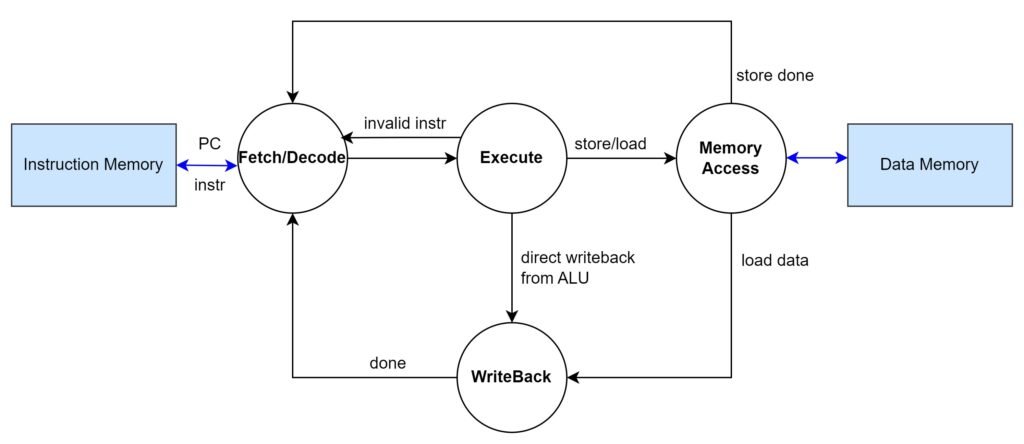
\includegraphics[width=1.0\textwidth]{./cpu1.jpg}
        \caption{CPU Organization: 5-Stage Pipeline}
    \end{figure}
    \begin{figure}[H] % Changed from [ht] to [H]
        \centering
        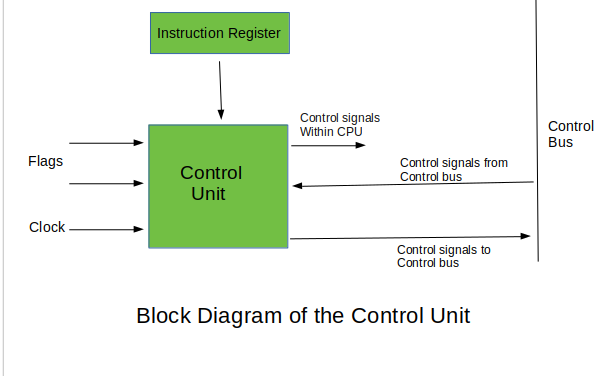
\includegraphics[width=1.0\textwidth]{./control_unit.png}
        \caption{Block Diagram Of Control Unit}
    \end{figure}

This register-based CPU design optimizes performance by leveraging registers, a flexible instruction format, and an efficient control unit. It balances trade-offs between speed, complexity, and memory efficiency, aligning with modern architectural principles while meeting the assignment’s objectives.

\section{Answers to Complex Problem-Solving Questions}
\begin{enumerate}
    \item \textbf{Efficient Instruction Execution Across Addressing Modes:} The register-based design with a flexible 32-bit format allows quick operand access (registers) and supports diverse modes (Immediate to Indexed), reducing memory bottlenecks.
    \item \textbf{Trade-offs Considered:} Larger instruction size enhances flexibility but increases fetch/decode complexity; mitigated by pipelining and a fast control unit.
    \item \textbf{Control Unit Management:} Parallel decoding and FSM sequencing ensure smooth handling of modes and pipeline stages.
    \item \textbf{Performance Challenges:} Data hazards and branch mispredictions are addressed with forwarding and prediction, though cache misses remain a limitation (assumes basic cache).
    \item \textbf{Alignment with Industry Standards:} The design mirrors modern RISC architectures (e.g., ARM) with register focus, pipelining, and flexible addressing, though it simplifies some features (e.g., no out-of-order execution).
\end{enumerate}


\end{document}